\documentclass[12pt]{beamer}

\newcommand{\emp}{\noindent\fboxsep=0pt}
\usefonttheme{serif}

\usetheme{Darmstadt}
\usepackage[utf8]{inputenc}
\usepackage[UTF8,zihao=-4]{ctexcap}
\usepackage[T1]{fontenc}
\usepackage{lmodern}
\usepackage{wrapfig}
\usepackage{fontspec}
\usepackage{color}
\usepackage{fancyhdr}
\usepackage{setspace}
\usepackage{caption}
\usepackage{mathptmx}
\usepackage{amsmath}
\usepackage{amssymb}
\usepackage{amstext}
\usepackage{geometry}
\usepackage{graphicx}
\usepackage{pifont}
\usepackage{float}
\usepackage{newclude}
\usepackage{subfig}
\usepackage{paralist}
\usepackage{booktabs} % 允许在表中使用\toprule、\ midrule和\ bottomrule% 定义正文字体
\usepackage[bookmarks=true]{hyperref}
\usepackage{tabularx}
%\usepackage{listings}


\setromanfont{Times New Roman}	% 将西文字体设置为 Times New Roman
% \setCJKfamilyfont{zhkai}{[SIMKAI.TTF]}
% \newcommand*{\kaiti}{\CJKfamily{zhkai}}

% 定义 caption
\DeclareCaptionFont{kaiticaption}{\kaishu \small}	% 定义下面三个caption的font的kaiticaption的具体格式
\captionsetup[figure]{font=small,labelsep=quad,skip=0.5ex,labelfont=bf,font=kaiticaption}	% 设置图片的 caption 格式 % 想要标题换行后居中,可以添加justification=centering
\captionsetup[table]{font=small,labelsep=quad,skip=0.5ex,labelfont=bf,font=kaiticaption}	% 设置表格的 caption 格式
\captionsetup[subfloat]{font=small,labelsep=quad,skip=0.5ex,labelfont=bf,font=kaiticaption}
\captionsetup[equation]{font=small,labelsep=quad,skip=0.5ex,labelfont=bf,font=kaiticaption}


% 设置图片,表格,公式编号格式
\renewcommand{\thetable}{\thesection{}-\arabic{table}}	% \thetable 表示设置的是表格的编号格式, 后面括号的内容为编号格式:章节号-表格的序号
\renewcommand{\thefigure}{\thesection{}-\arabic{figure}}
\renewcommand{\theequation}{\thesection{}-\arabic{equation}}


% 设置代码块
%\definecolor{commentcolor}{RGB}{85,139,78}
%\definecolor{stringcolor}{RGB}{206,145,108}
%\definecolor{keywordcolor}{RGB}{34,34,250}
%\lstset{
%	language=Matlab, % 默认代码语言.
%	basicstyle=\footnotesize,
%	numbers=left, %设置行号位置
%	numberstyle=\tiny, %设置行号大小
%	commentstyle=\color{commentcolor},	%注释颜色
%	keywordstyle=\color{keywordcolor},	%关键词颜色
%	stringstyle=\color{stringcolor},	%字符串颜色
%	frame=single, %设置边框格式
%	escapeinside=``, %逃逸字符(1左面的键),用于显示中文
%	breaklines = True, % 自动折行
%	breakatwhitespace = True, % 自动折行时打断单词
%	extendedchars=false, %解决代码跨页时,章节标题,页眉等汉字不显示的问题
%	xleftmargin=2em,xrightmargin=2em, aboveskip=1em, %设置边距
%	tabsize=4, %设置tab空格数
%	showspaces=false %不显示空格
%}

\graphicspath{{../img/}}
\useoutertheme{split}
\setbeamertemplate{headline}{}
\begin{document}
\abovedisplayshortskip=0pt	%设置公式距离上方非重叠区域额外添加的距离,推荐0
\belowdisplayshortskip=0pt
\abovedisplayskip=0pt	%设置公式距离上方重叠距离额外添加的距离,推荐0
\belowdisplayskip=0pt
% 下面两行用于删除导航栏

% 当前section起始页
\section{Automobile Overview}
\begin{frame}
	\centering\Huge\textbf{Automobie Overview}
\end{frame}
% 当前subsection第一页
\subsection{Types}
\begin{frame}{Types}	% 括号里填subsection
	\begin{block}{categorized by use} % subsubsection
		\begin{figure}[htbp]
			\centering
			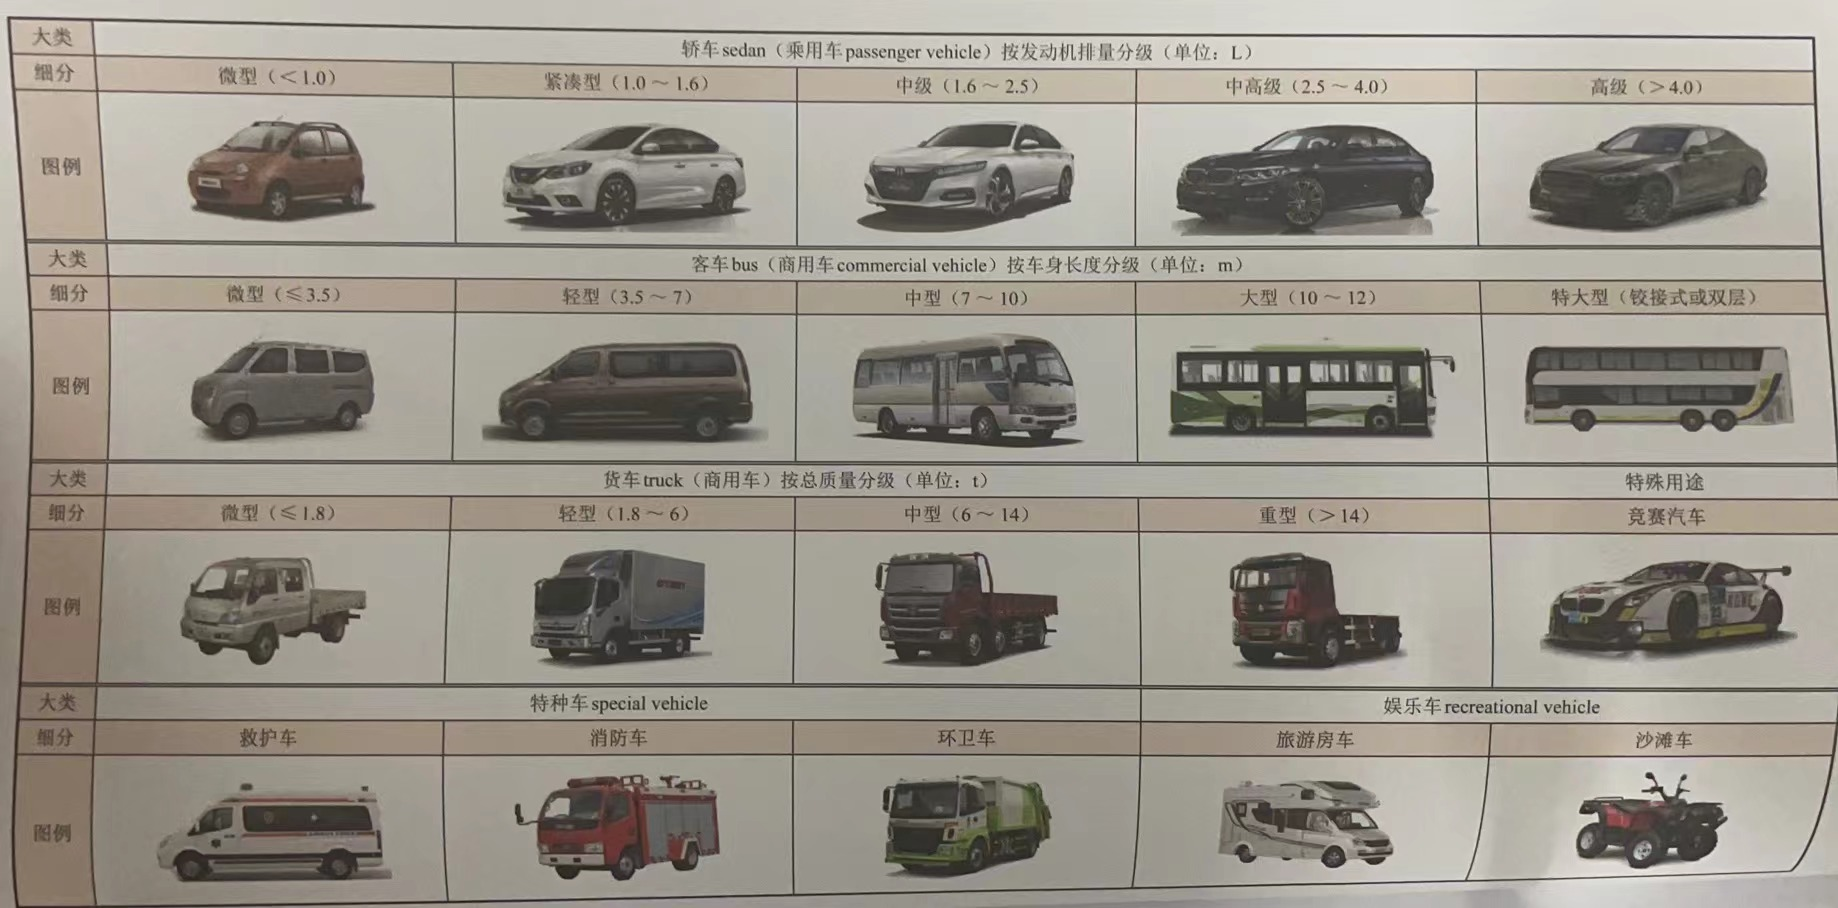
\includegraphics[width=1\textwidth]{1-1}
		\end{figure}
	\end{block}
\end{frame}
\begin{frame}	% 当前subsection的第二页
	\begin{block}{catogorized by body}
		\begin{figure}[htbp]
			\centering
			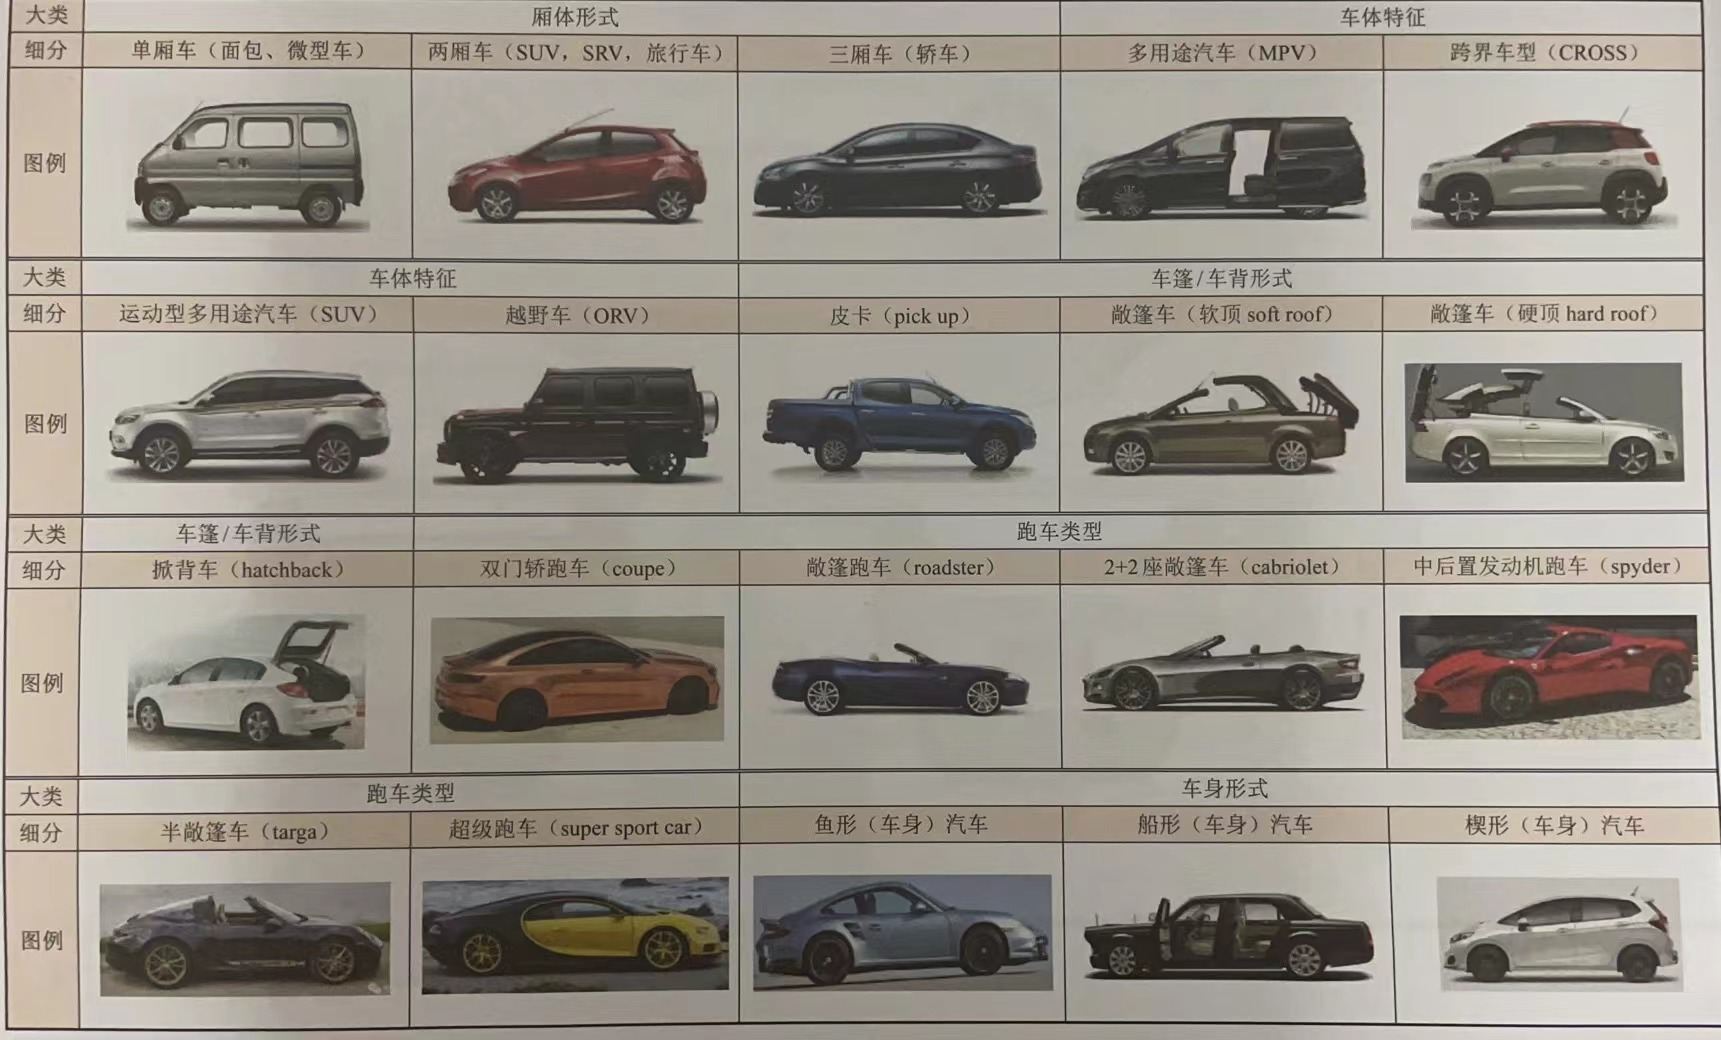
\includegraphics[width=1\textwidth]{1-2}
		\end{figure}
	\end{block}
\end{frame}
\subsection{parameters}
\begin{frame}{parameters}
	\begin{block}{body}
		\begin{compactitem}
			\item front track: the distance between the front wheel centerlines
			\item rear track
			\item turning radius: the distance between a outer wheel center plane and its turning center
			\item minimum turning radius: the turning radius when a steering wheel is turned to its limit position
			\item front hang: the distance between a car's head and the center of the front axel
			\item rear hang: the distance between a car's butt and the center of the rear axel
			\item wheelbase: the distance between the front and rear axels
		\end{compactitem}
	\end{block}
\end{frame}
\begin{frame}
	\begin{block}{}
		\begin{compactitem}
			\item approaching and departure angle
			\begin{figure}[htbp]
				\centering
				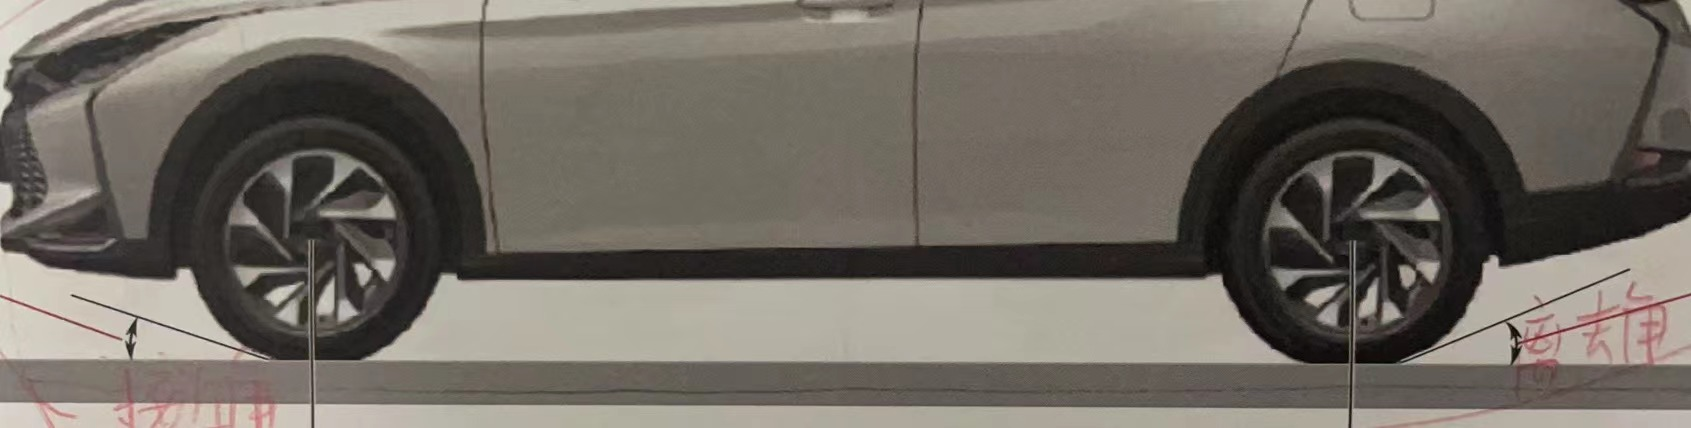
\includegraphics[width=0.8\textwidth]{1-3}
			\end{figure}
		\end{compactitem}
	\end{block}
\end{frame}
\begin{frame}
	\begin{block}{Performance}
		\begin{compactitem}
			\item maximum climbing angle: maximum climbing angle when fully loaded
			\item maximum tilt angle:
				\begin{figure}[htbp]
					\centering
					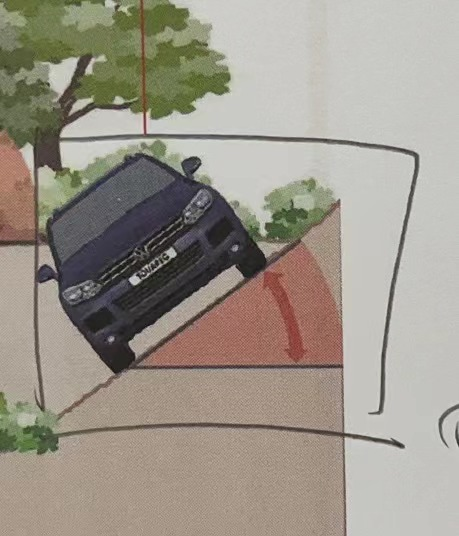
\includegraphics[width=0.1\textwidth]{1-4}
				\end{figure}
			\item  through angle :
				\begin{figure}[htbp]
					\centering
					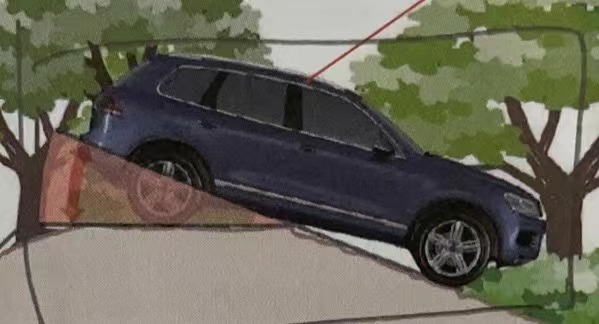
\includegraphics[width=0.1\textwidth]{1-5}
				\end{figure}
			\item maximum wading depth
			\item maximum speed: maximum speed when a car drives on a flat road
			\item vehicle equipment quality: mass when fully equipped with all items
			\item maximum total mass: mass when fully loaded
			\item average fuel consumption(L/100km)
		\end{compactitem}
	\end{block}
\end{frame}
\begin{frame}
	\begin{block}{}
		\begin{compactitem}
			\item maximum axle load mass: the max mass a single axel can bear
			\item 100km acceleration: the shortest time for a car to accelerate from 0 to 100 km/h
			\item breaking distance: the shortes distance for a car to decelerate from 100km/h to 0
			\item number of wheels and drive wheels(n $\times$ m): n = number of wheels, m = number of drive wheels
		\end{compactitem}
	\end{block}
\end{frame}
\subsection{Automobile Components}
\begin{frame}{Automobile Components}
	\begin{block}{overview}
		A automobile is usually composed of power, chassis, body and electrical systems
		\begin{figure}[htbp]
			\centering
			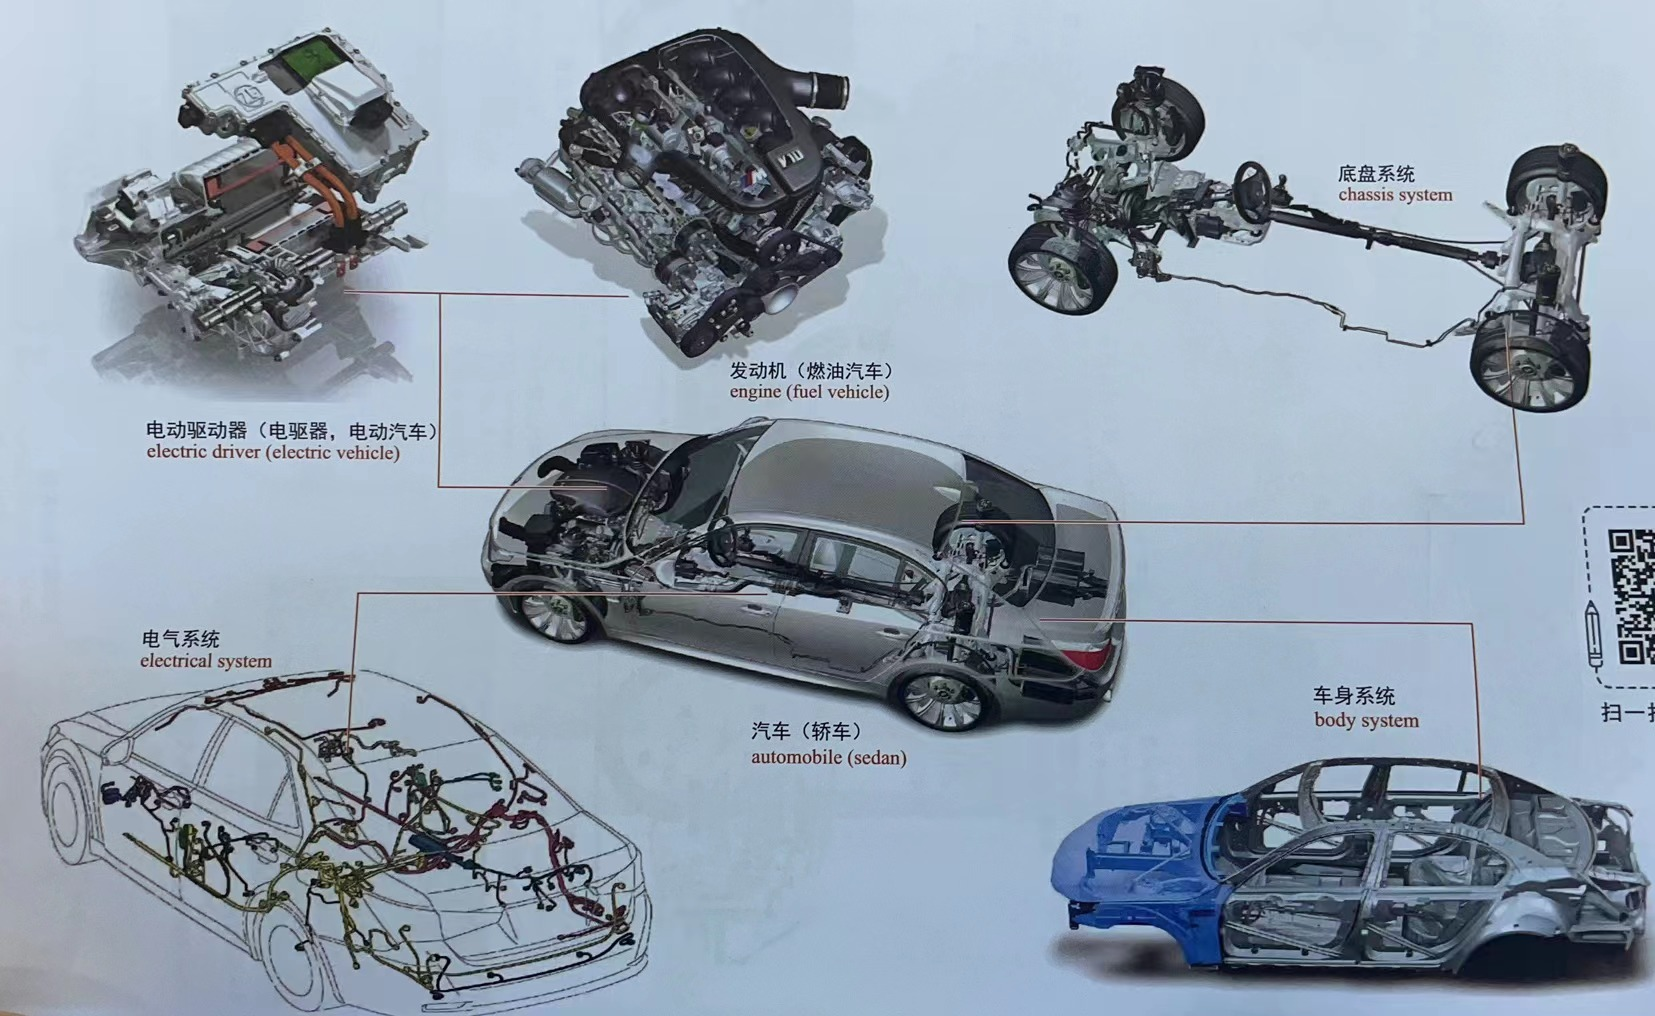
\includegraphics[width=0.8\textwidth]{1-6}
		\end{figure}
	\end{block}
\end{frame}
\begin{frame}
	\begin{block}{power}
		\begin{compactitem}
			\item ICE(internal combustion engine)
				\begin{figure}[htbp]
					\centering
					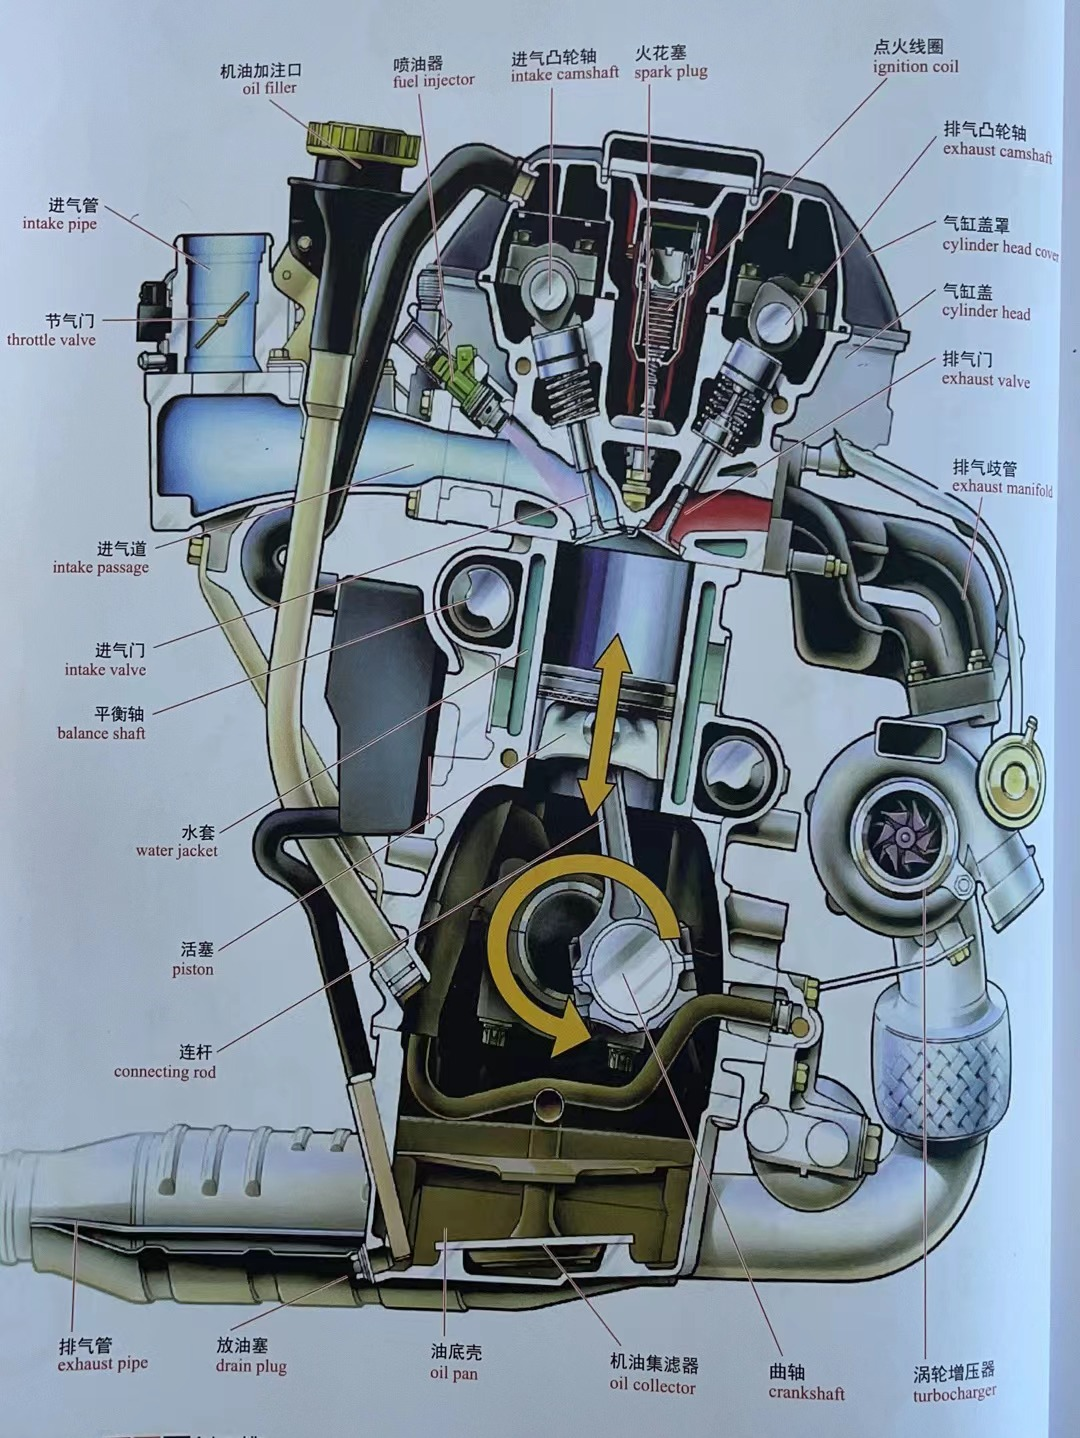
\includegraphics[width=0.5\textwidth]{1-7}
				\end{figure}
		\end{compactitem}
	\end{block}
\end{frame}
\begin{frame}
	\begin{block}{}
		\begin{compactitem}
			\item electric drive assembly
			
			{\footnotesize usually composed of drive motor, reducer and MCU 
				
				can also integrate PDU, DC/DC, DC/AC, OBC, BMC and VCU}
				\begin{figure}[htbp]
					\centering	
					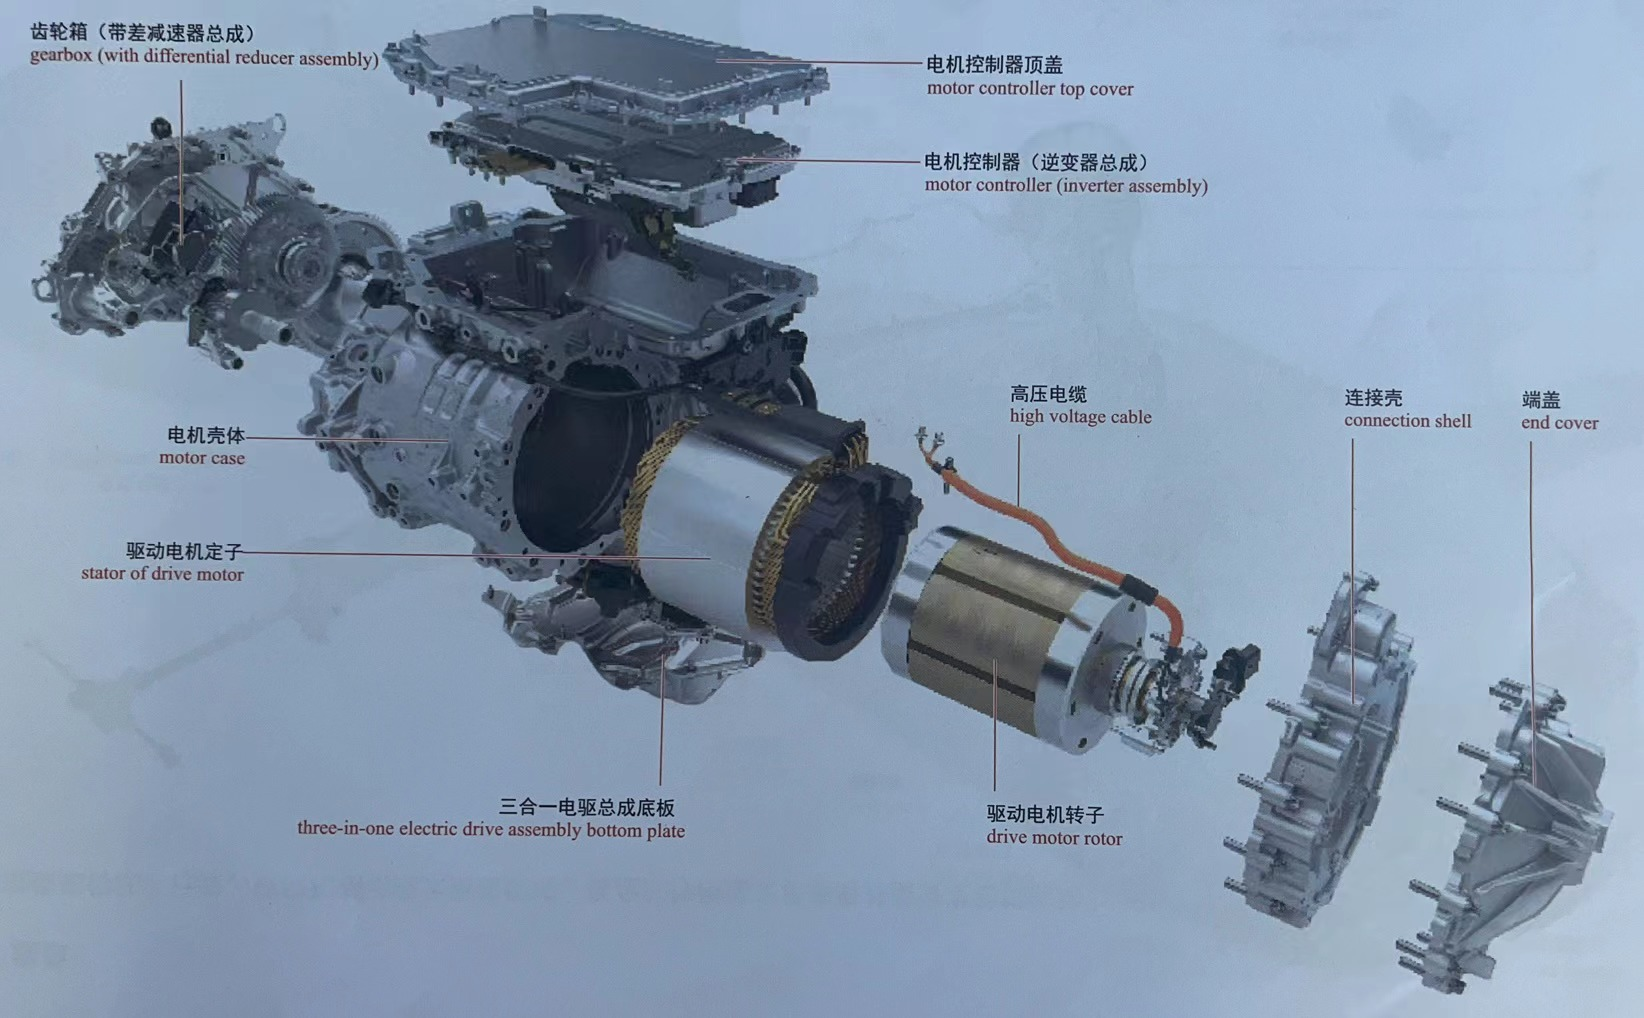
\includegraphics[width=0.8\textwidth]{1-8}
				\end{figure}
		\end{compactitem}
	\end{block}
\end{frame}
\begin{frame}
	\begin{block}{}
		{
			\footnotesize
			\begin{align*}
				& \text{MCU: motor control unit} & &\text{PDU: power control unit} \\
				& \text{OBC: on board charger} & &\text{BMS: battery management system} \\
				& \text{VCU: vehicle control unit} \\
			\end{align*}
		}
	\end{block}
\end{frame}
\begin{frame}
	\begin{block}{chassis}
		a chasis is composed of transmission, driving, steering and breaking systems
		\begin{figure}[htbp]
			\centering
			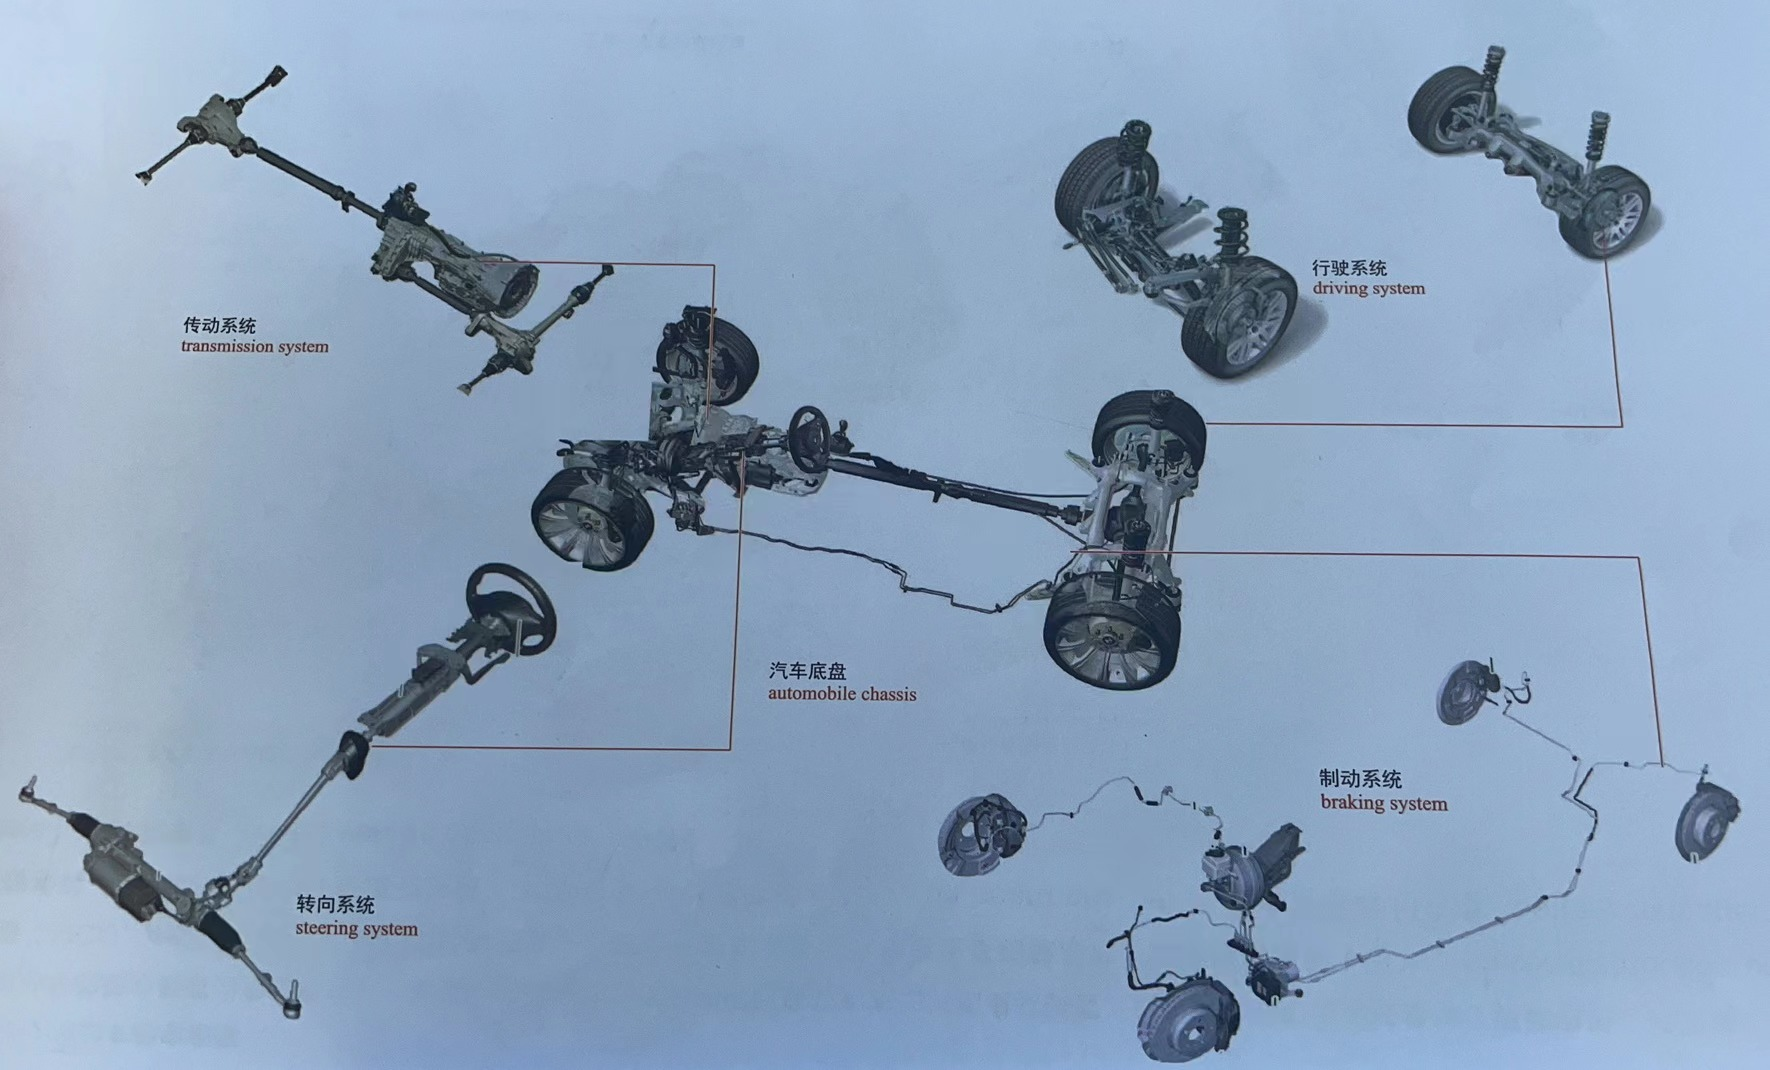
\includegraphics[width=0.9\textwidth]{1-9}
		\end{figure}
	\end{block}
\end{frame}
\begin{frame}
	\begin{block}{}
		\begin{figure}[htbp]
			\centering
			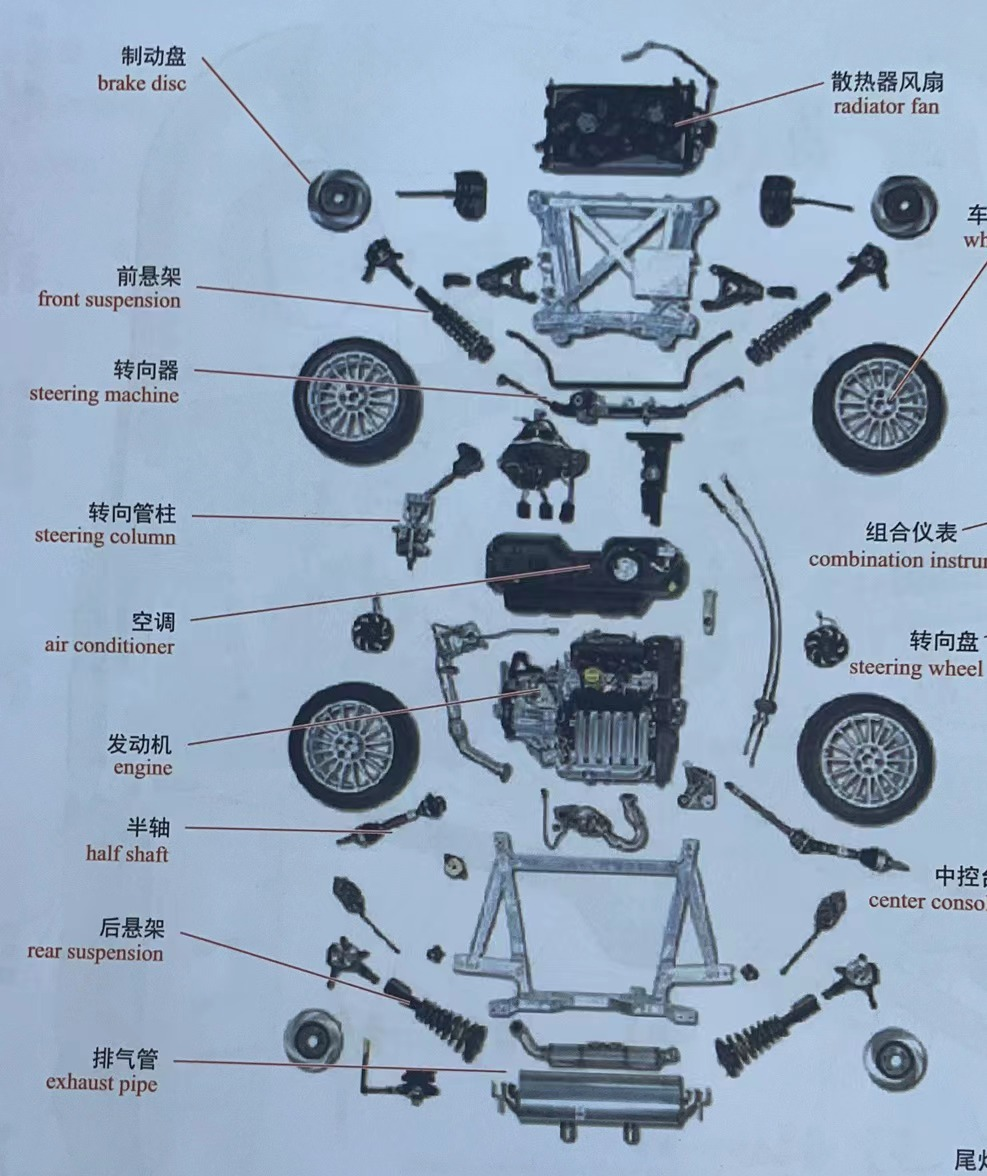
\includegraphics[width=0.6\textwidth]{1-10}
		\end{figure}
	\end{block}
\end{frame}
\begin{frame}
	\begin{block}{body}
		\begin{figure}[htbp]
			\centering
			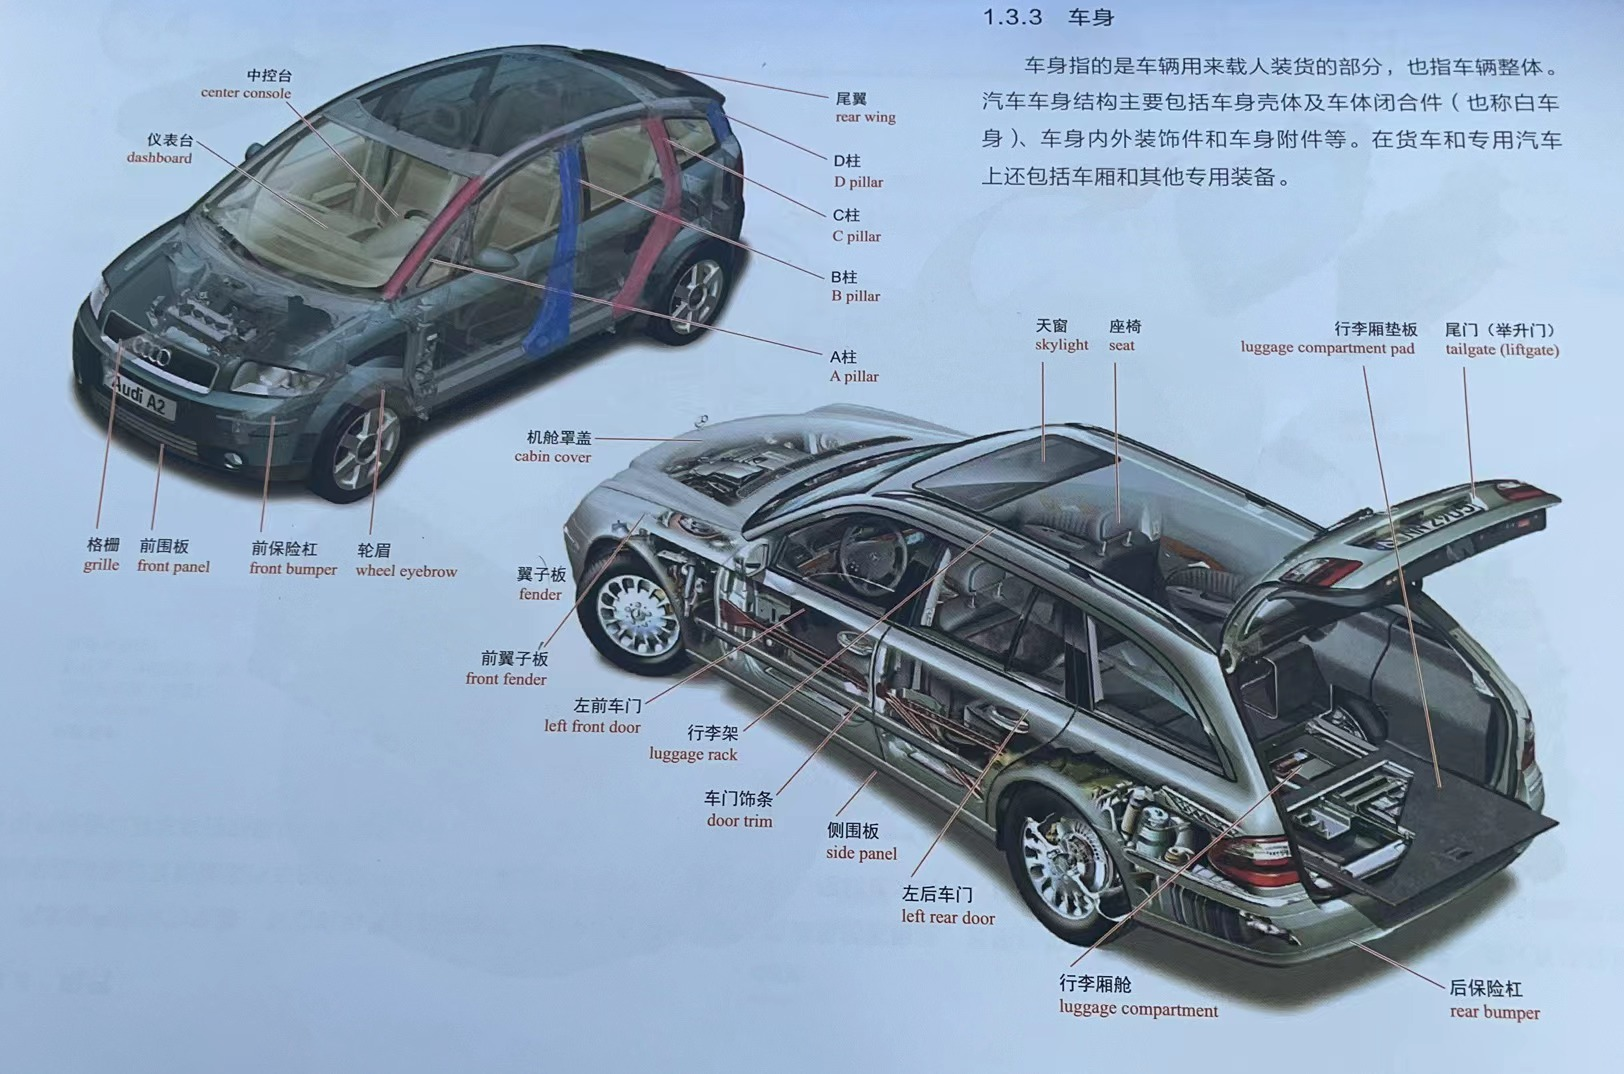
\includegraphics[width=0.8\textwidth]{1-11}
		\end{figure}
	\end{block}
\end{frame}
\begin{frame}
	\begin{block}{}
		\begin{figure}[htbp]
			\centering
			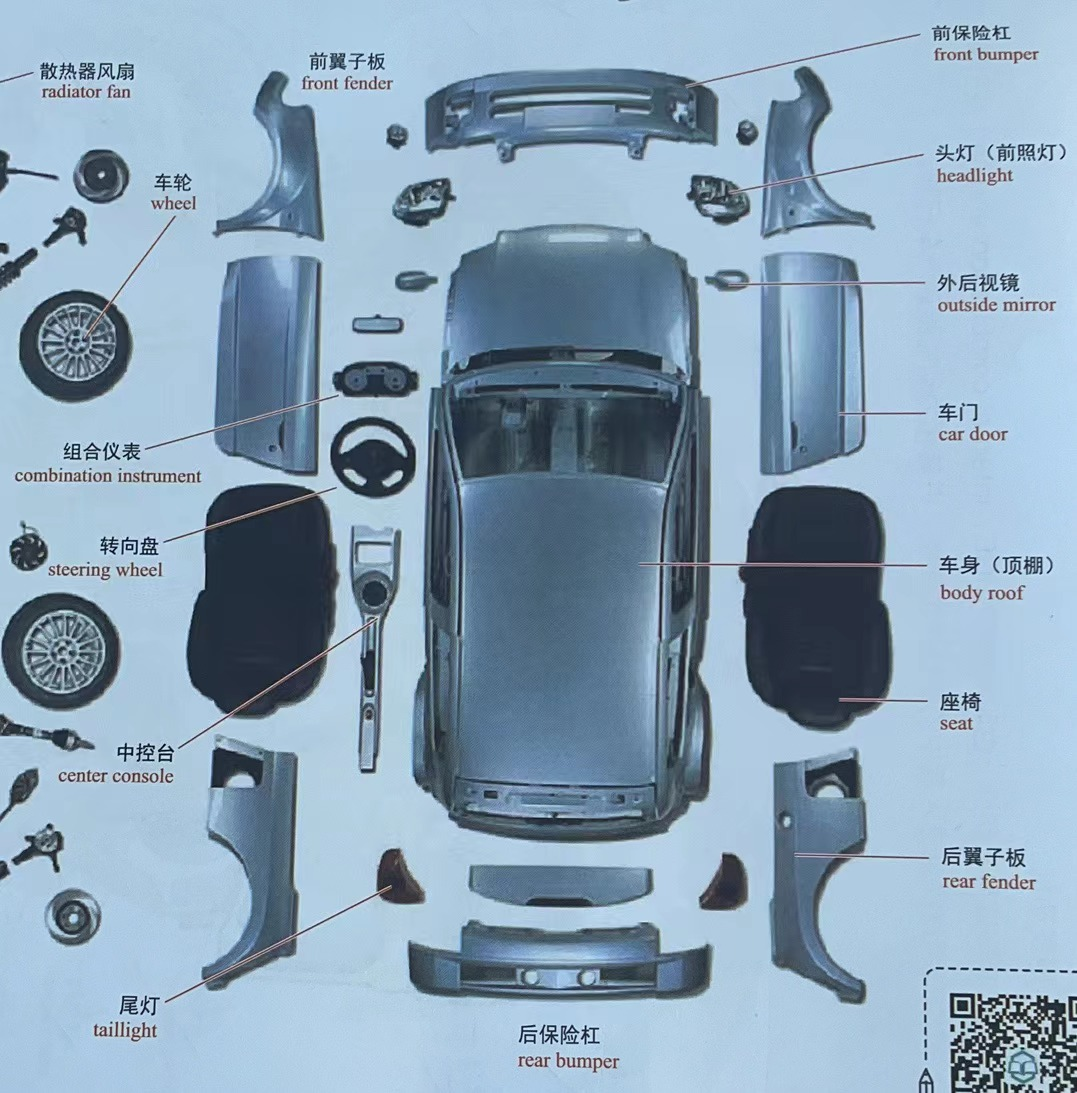
\includegraphics[width=0.7\textwidth]{1-12}
		\end{figure}
	\end{block}
\end{frame}
\begin{frame}
	\begin{block}{electrical system}
		The electrical system is composed of power, engine electrical, chassis electrical, body electrical systems
		\begin{figure}[htbp]
			\centering
			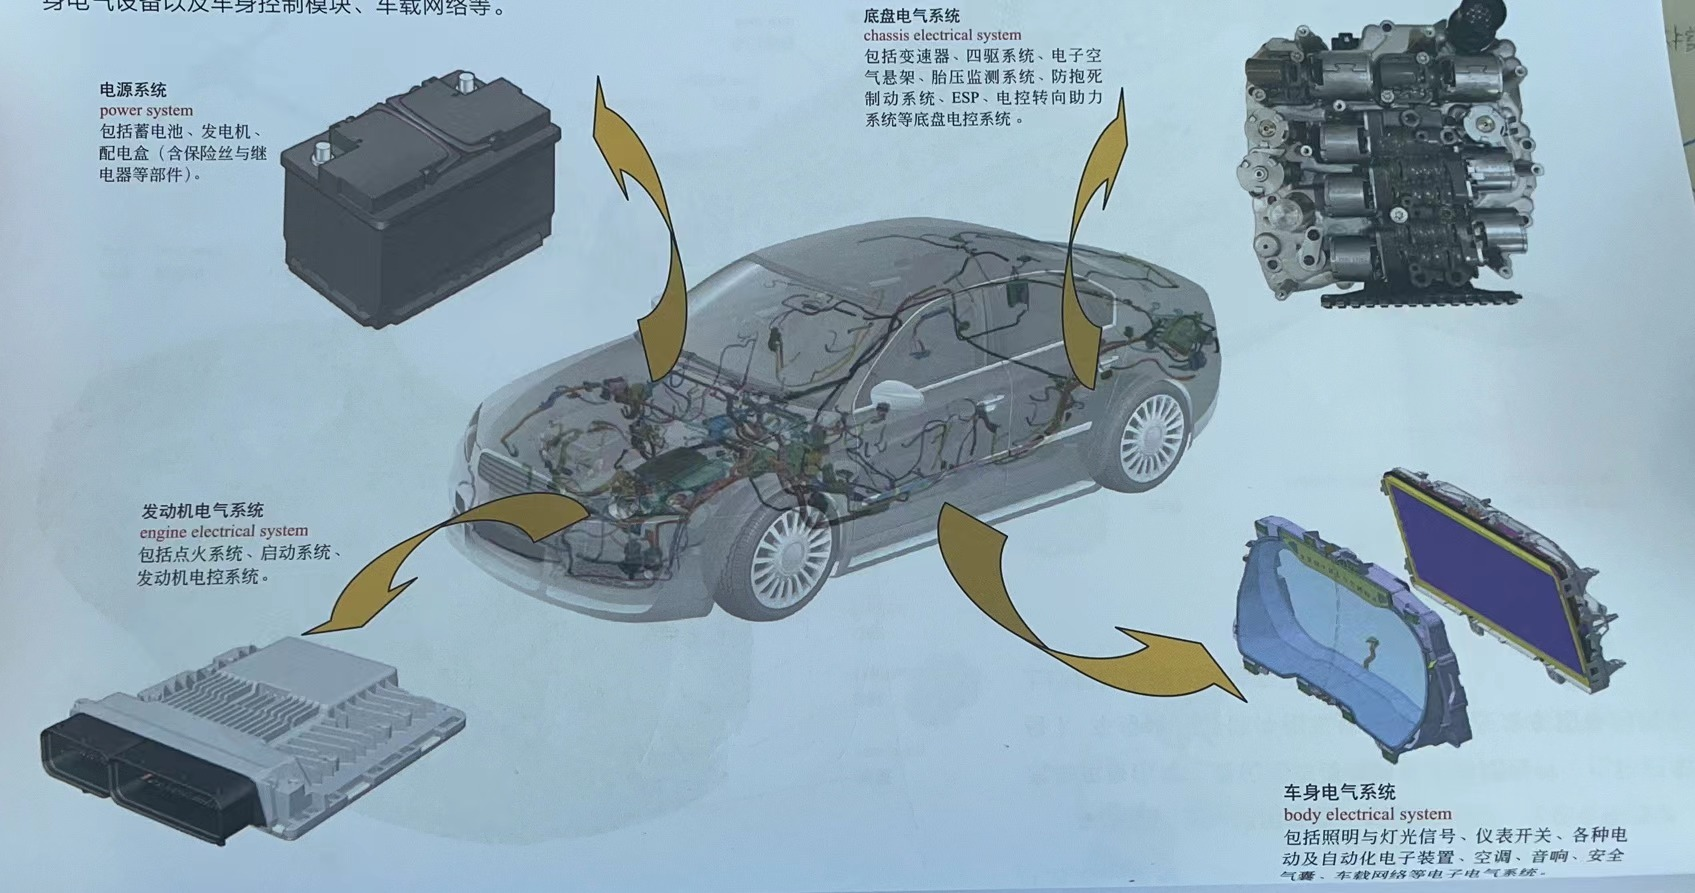
\includegraphics[width=0.8\textwidth]{1-13}
		\end{figure}
	\end{block}
\end{frame}
\subsection{Automobile Principles}
\begin{frame}{Automobile Principles}
	\begin{block}{ICE vehicle}
		\begin{compactitem}
			\item structure
			\begin{figure}[htbp]
				\centering
				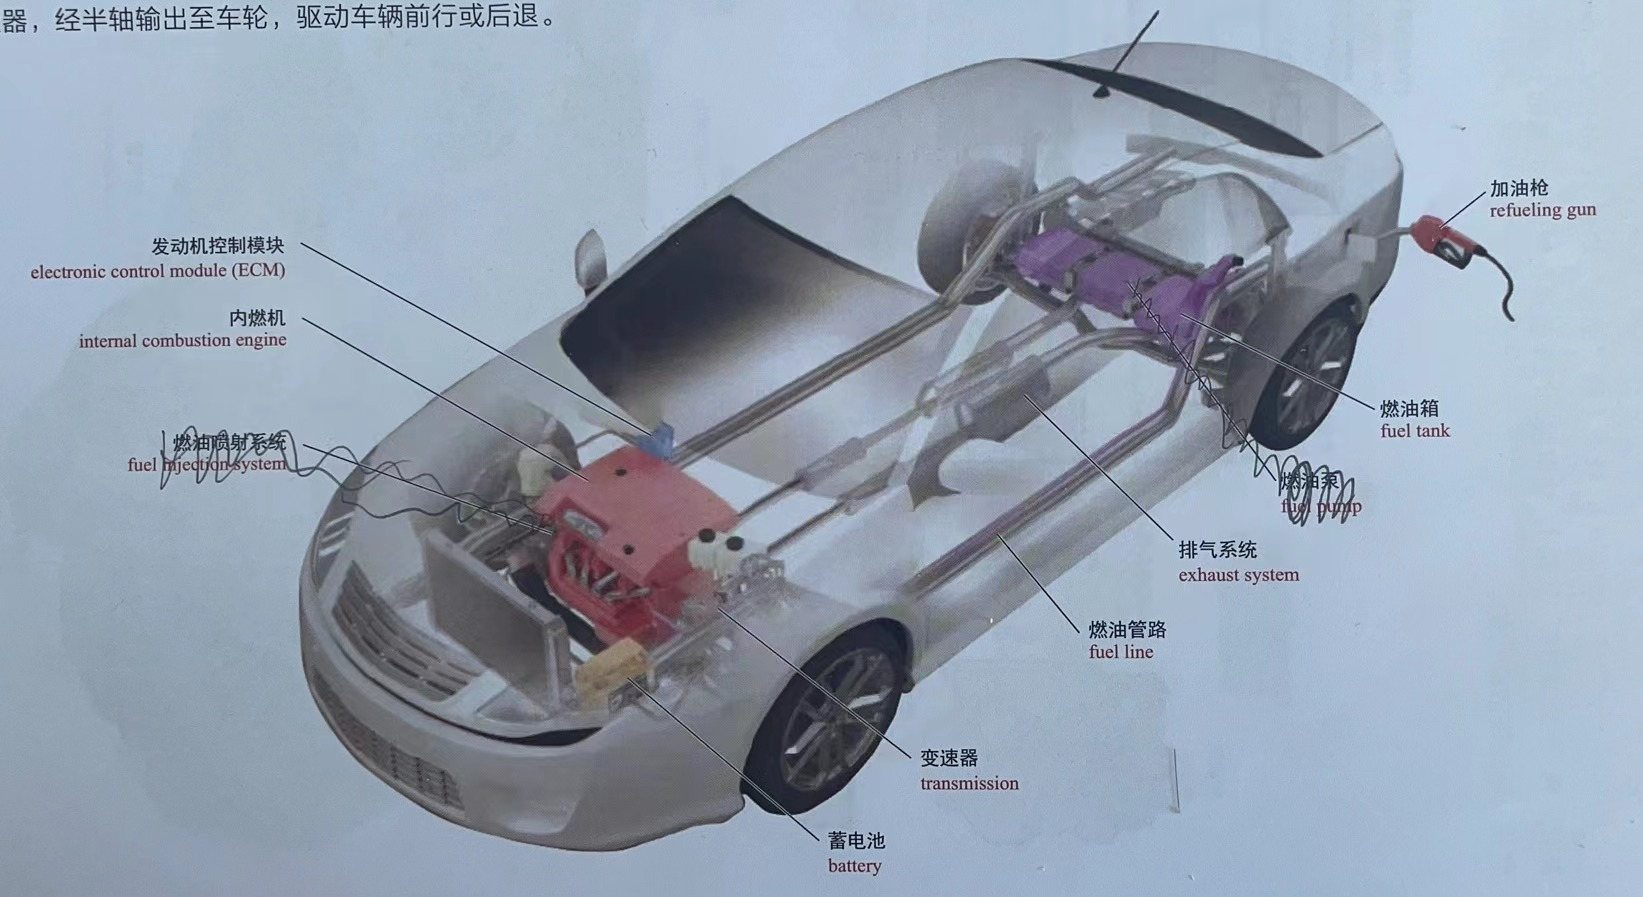
\includegraphics[width=0.8\textwidth]{1-14}
			\end{figure}
		\end{compactitem}
	\end{block}
\end{frame}
\begin{frame}
	\begin{block}{}
		\begin{compactitem}
			\item principle
			\begin{figure}[htbp]
				\centering
				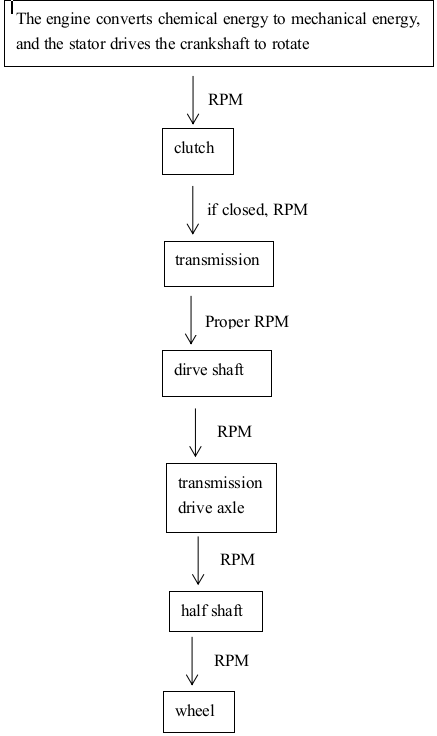
\includegraphics[width=0.35\textwidth]{1-15}
			\end{figure}
		\end{compactitem}
	\end{block}
\end{frame}
\begin{frame}
	\begin{block}{HEV(hybrid-electric-vehicle)}
		\begin{compactitem}
			\item structure
			\begin{figure}[htbp]
				\centering
				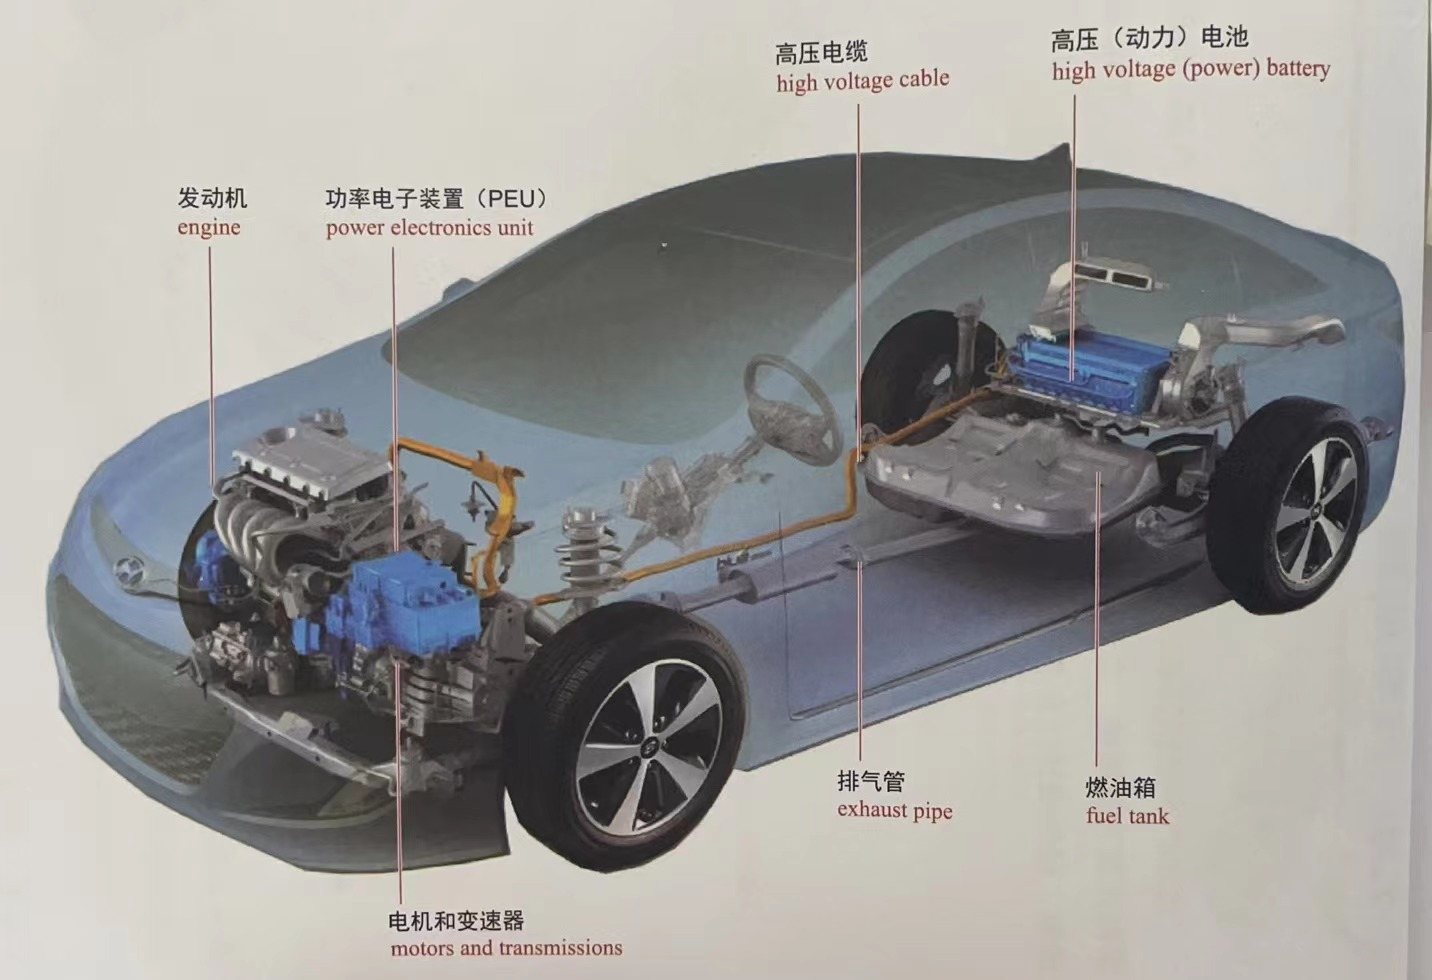
\includegraphics[width=0.5\textwidth]{1-16}
			\end{figure}
		\end{compactitem}
	\end{block}
\end{frame}
\begin{frame}
	\begin{block}{}
		\begin{compactitem}
			\item principle
				\begin{figure}[htbp]
					\centering
					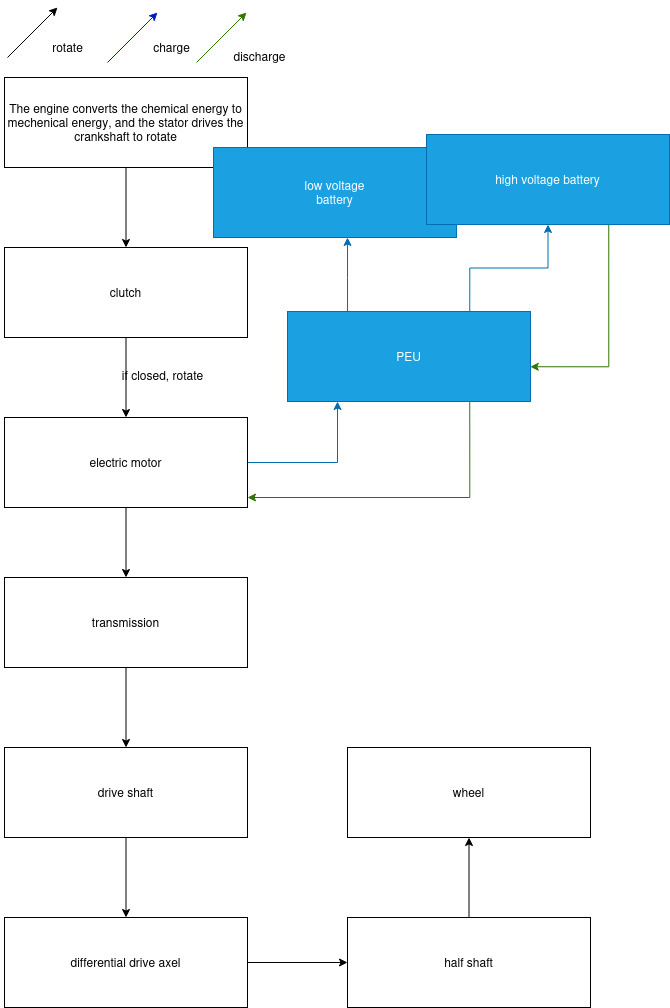
\includegraphics[width=0.4\textwidth]{1-17}
				\end{figure}
		\end{compactitem}
	\end{block}
\end{frame}
\begin{frame}
	\begin{block}{PHEV(plug-in hybrid electric vehicle)}
		\begin{compactitem}
			\item features: pure electric mode, hybrid mode
			\item structure:
				\begin{figure}[htbp]
					\centering
					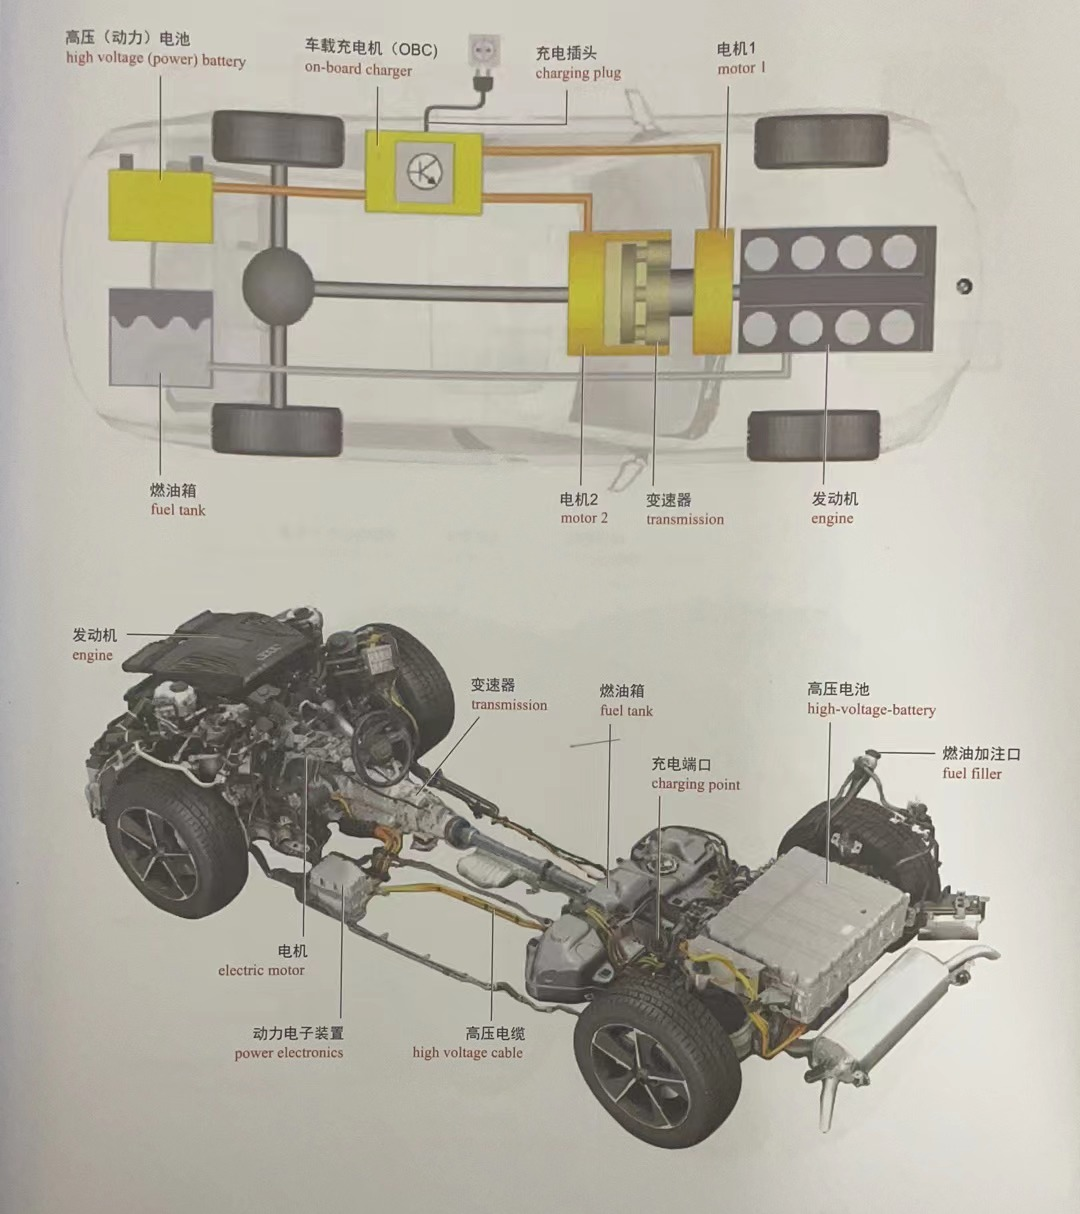
\includegraphics[width=0.5\textwidth]{1-18}
				\end{figure}
		\end{compactitem}		
	\end{block}
\end{frame}
\begin{frame}
	\begin{block}{REEV(range extend electric vehicle)}
		\begin{compactitem}
			\item features :
			\begin{compactenum}
				\item if fully charged, pure electric mode
				\item if the electricity insufficient, the motor drives the generator to charge the high voltage battery
				\item when braking or decelerating for overspeeding, charge the high voltage battery
			\end{compactenum}
		\end{compactitem}
	\end{block}
\end{frame}
\begin{frame}
	\begin{block}{}
		\begin{compactitem}
			\item structure
				\begin{figure}[htbp]
					\centering
					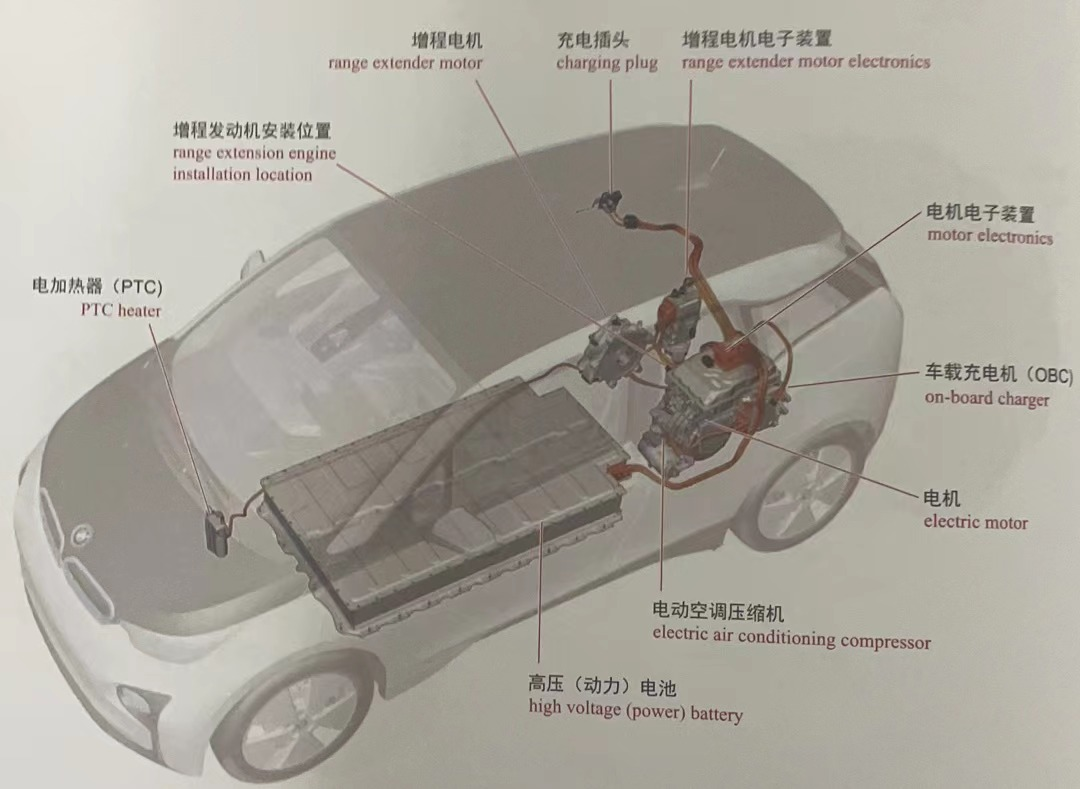
\includegraphics[width=0.8\textwidth]{1-19}
				\end{figure}
		\end{compactitem}
	\end{block}
\end{frame}
\begin{frame}
	\begin{block}{}
		\begin{compactitem}
			\item principle
				\begin{figure}[htbp]
					\centering
					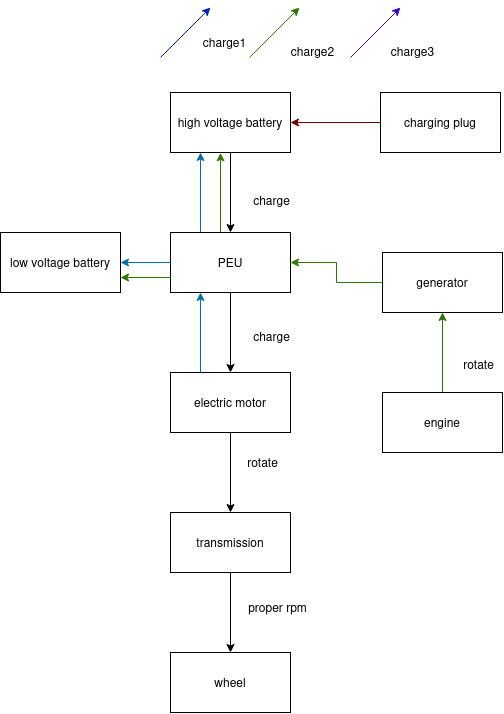
\includegraphics[width=0.4\textwidth]{1-20}
				\end{figure}
		\end{compactitem}
	\end{block}
\end{frame}
\begin{frame}
	\begin{block}{BEV(battery electric vehicle)}
		\begin{compactitem}
			\item structure
				\begin{figure}[htbp]
					\centering
					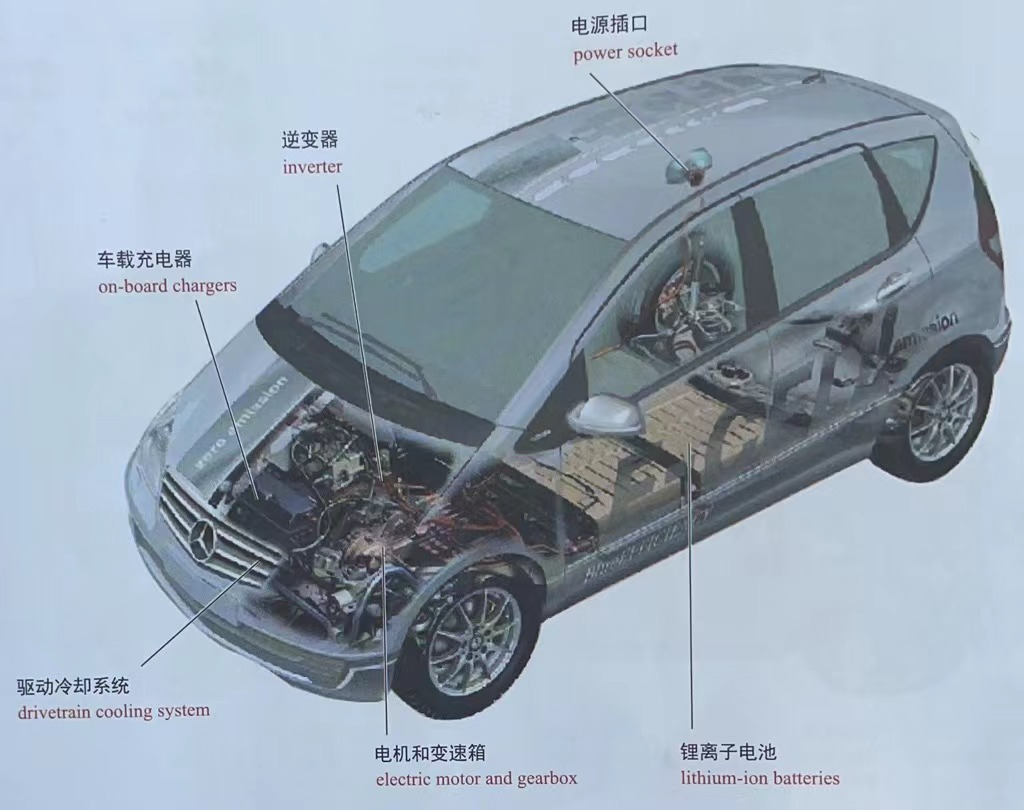
\includegraphics[width=0.8\textwidth]{1-21}
				\end{figure}
		\end{compactitem}
	\end{block}
\end{frame}
\begin{frame}
	\begin{block}{}
		\begin{compactitem}
			\item principle
			\begin{figure}[htbp]
				\centering
				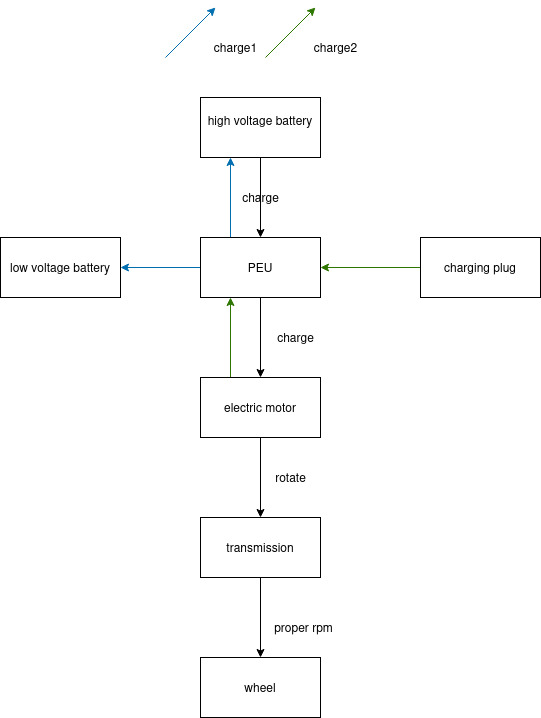
\includegraphics[width=0.4\textwidth]{1-22}
			\end{figure}
		\end{compactitem}
	\end{block}
\end{frame}
\begin{frame}
	\begin{block}{FCEV(fuel cell electric vehicle)}
		\begin{compactitem}
			\item structure
			\begin{figure}[htbp]
				\centering
				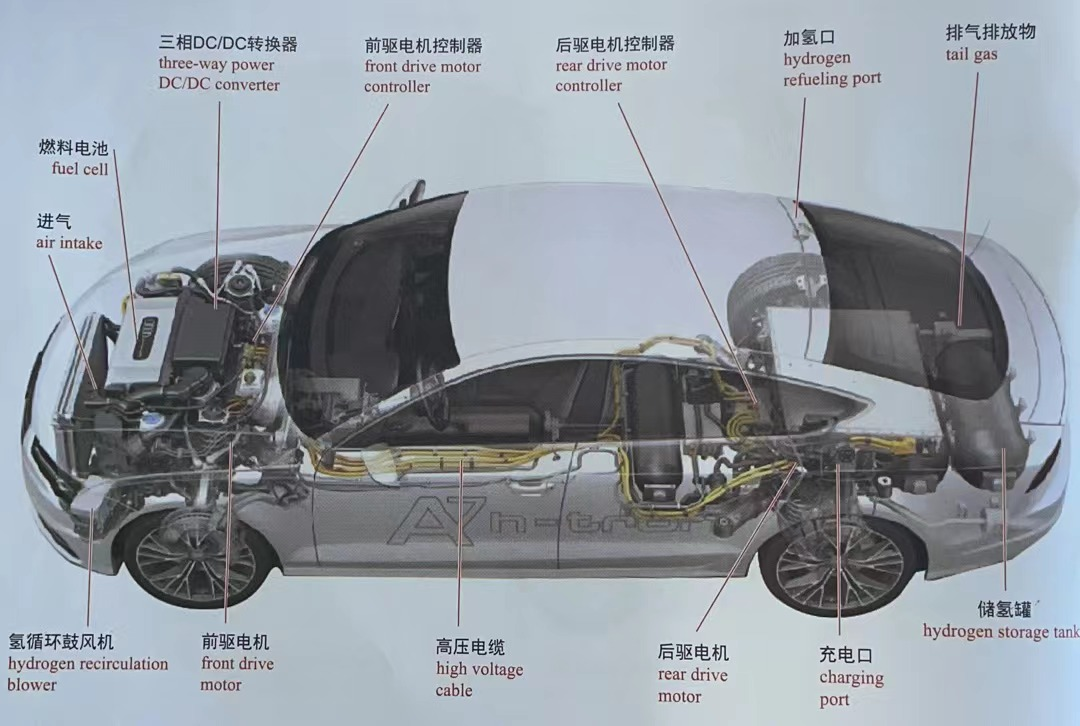
\includegraphics[width=0.8\textwidth]{1-23}
			\end{figure}			
		\end{compactitem}
	\end{block}
\end{frame}
\begin{frame}
	\begin{block}{}
		\begin{compactitem}
			\item principle
			\begin{figure}[htbp]
				\centering
				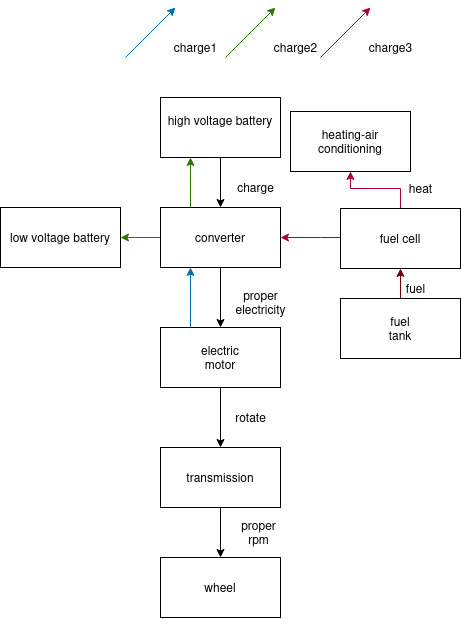
\includegraphics[width=0.4\textwidth]{1-24}
			\end{figure}
		\end{compactitem}
	\end{block}
\end{frame}
\end{document}




iffalse
\begin{frame}
	\begin{block}{}
		\begin{compactitem}
			\item 
		\end{compactitem}
	\end{block}
\end{frame}
%%%%%%%%%
\begin{frame}
	\begin{block}{}
		\begin{compactitem}
			\item 
			\begin{figure}[htbp]
				\centering
				\includegraphics[width=\textwidth]{imagefile}
			\end{figure}
		\end{compactitem}
	\end{block}
\end{frame}
if